\documentclass{article}
\usepackage[utf8]{inputenc}
\usepackage{graphicx}


\begin{document}



\begin{enumerate}
    \item \textbf{Derive formula of $L_{2}(x)$ in terms of interpolation phase $ u = \frac{x - x_{i}}{h} $. Integrate $ \hat{I_{i}^{i+2}}$ with received formula as integrand [mathematical formula].}
    
    $$
    L_2(x) = \frac{(x-x_{i+1})(x-x_{i+2})}{(x_i-x_{i+1})(x_i-x_{i+2})}f_i + 
    \frac{(x-x_{i})(x-x_{i+2})}{(x_{i+1}-x_{i})(x_{i+1}-x_{i+2})}f_{i+1} + 
    \frac{(x-x_{i+1})(x-x_i)}{(x_{i+2}-x_i)(x_{i+2}-x_{i+1})}f_{i+2}
    $$
    Let's substitute this equation with  $u=\frac{x-x_i}{h}$
    
    Using a fact, that $x_{i+1} = x_i+h$ and $x_{i+2} = x_i+2h$
    we'll end up with equation:
    
   $ L_2(x)=\frac{1}{2}(u^2-3u+2)f_i + (2u-u^2)f_{i+1} + \frac{1}{2}(u^2-u)f_{i+2}$
   
   Integrating it with respect to u($du = \frac{dx}{h}, hdu = dx$, also don't forget to change interpolation borders ${a, b}$ from $x_{i+2}$ and $x_{i}$ to $u(a) = 2$, $u(b) = 0$
   
   Solving that integral will result in Simpson's formula:
   
    $\hat{I}^{i+2}_{i} = \frac{h}{3}(f_i+4f_{i+1}+f_{i+2})$
    
    \item \textbf{Explain how used condition $n = 2k$ helps us in integration. If we want to use odd number of segments we have to integrate with even number of segments but add the value $I_{n-1}^n$. What is the calculation accuracy order of $I_{n-1}^n$? Why? Explain both.}
    
    If number of segments is even, we are able to construct non-overlapping 3-point-template interpolant - every two adjacent segments consist of 3 points. Odd number of segments leaves one of them without its complement to three-point-template.
    
    We solve this problem by at first computing even number of segments' integrals and then adding the last one, computed by some other means. N.B. that it must be computed with error of at least $O(h^4)$ - in this case our total error would remain O($h^4$).
    
    We can do that with, for example
    
    $\hat{I}^{n}_{n-1} = \frac{3h}{8}(f_{n-3}+3f_{n-2}+3f_{n-1}+f_n)$
    
    which has $O(h^5)$ error estimation.
    
    
    \item \textbf{Derive the formula of whole $\hat{I_{a}^{b}}$. Summarize all integrals on segments $\hat{I_{i}^{i+1}}$ for even case, and for odd case. [mathematical formula]}
    
    For even n - number of segments:
    
    $\hat{I}^{b}_{a} = \sum_{i=0}^{n/2-1} \hat{I}^{2(i+1)}_{2i}$
    
    for even n:
    
    $\hat{I}^{b}_{a} = \sum_{i=0}^{(n-1)/2-1} \hat{I}^{2(i+1)}_{2i} + I^n_{n-1}$
    
    \item \textbf{Derive the formula of trapezoid quadrature formula error estimation. Use Taylor series expansion for antiderivative $F_{i+1}$ and $f_{i+1}$ [mathematical formula]}
    
    
    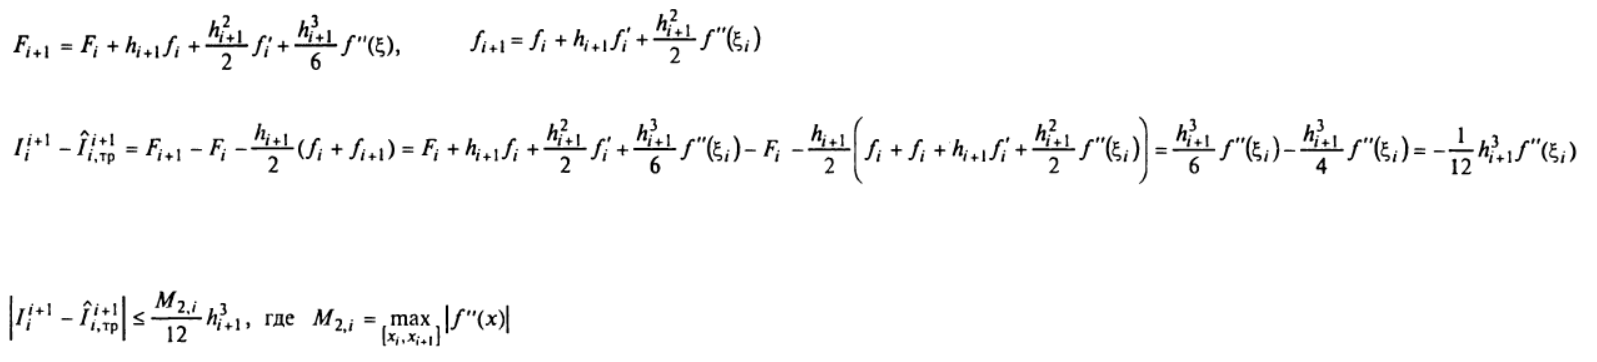
\includegraphics[scale=0.25]{q4answer.png}
\end{enumerate}

\end{document}
